\documentclass[letterpaper,11pt]{article}

\usepackage{latexsym}
\usepackage[empty]{fullpage}
\usepackage{titlesec}
\usepackage{marvosym}
\usepackage[usenames,dvipsnames]{color}
\usepackage{verbatim}
\usepackage{enumitem}
\usepackage[hidelinks]{hyperref}
\usepackage{fancyhdr}
\usepackage[english]{babel}
\usepackage{tabularx}
\usepackage{fontawesome5}
\usepackage{multicol}
\setlength{\multicolsep}{-3.0pt}
\setlength{\columnsep}{-1pt}
\input{glyphtounicode}

%new packages

\usepackage{fontenc}
\usepackage{amsmath}
\usepackage{amssymb}
\usepackage{graphicx}



%----------FONT OPTIONS----------

\pagestyle{fancy}
\fancyhf{} % clear all header and footer fields
\fancyfoot{}
\renewcommand{\headrulewidth}{0pt}
\renewcommand{\footrulewidth}{0pt}

% Adjust margins
\addtolength{\oddsidemargin}{-0.6in}
\addtolength{\evensidemargin}{-0.5in}
\addtolength{\textwidth}{1.19in}
\addtolength{\topmargin}{-.7in}
\addtolength{\textheight}{1.4in}

\urlstyle{same}

\raggedbottom
\raggedright
\setlength{\tabcolsep}{0in}

% Sections formatting
\titleformat{\section}{
  \vspace{-4pt}\scshape\raggedright\large\bfseries
}{}{0em}{}[\color{black}\titlerule \vspace{-5pt}]



% Ensure that generate pdf is machine readable/ATS parsable
\pdfgentounicode=1

%-------------------------
% Custom commands
\newcommand{\resumeItem}[1]{
  \item\small{
    {#1 \vspace{-2pt}}
  }
}

\newcommand{\classesList}[4]{
    \item\small{
        {#1 #2 #3 #4 \vspace{-2pt}}
  }
}

\newcommand{\resumeSubheading}[4]{
  \vspace{-2pt}\item
    \begin{tabular*}{1.0\textwidth}[t]{l@{\extracolsep{\fill}}r}
      \textbf{#1} & \textbf{\small #2} \\
      \textit{\small#3} & \textit{\small #4} \\
    \end{tabular*}\vspace{-7pt}
}

\newcommand{\resumeSubSubheading}[2]{
    \item
    \begin{tabular*}{0.97\textwidth}{l@{\extracolsep{\fill}}r}
      \textit{\small#1} & \textit{\small #2} \\
    \end{tabular*}\vspace{-7pt}
}

\newcommand{\resumeProjectHeading}[2]{
    \item
    \begin{tabular*}{1.001\textwidth}{l@{\extracolsep{\fill}}r}
      \small#1 & \textbf{\small #2}\\
    \end{tabular*}\vspace{-7pt}
}


\newcommand{\resumeSubItem}[1]{\resumeItem{#1}\vspace{-4pt}}

\renewcommand\labelitemi{$\vcenter{\hbox{\tiny$\bullet$}}$}
\renewcommand\labelitemii{$\vcenter{\hbox{\tiny$\bullet$}}$}

\newcommand{\resumeSubHeadingListStart}{\begin{itemize}[leftmargin=0.0in, label={}]}
\newcommand{\resumeSubHeadingListEnd}{\end{itemize}}
\newcommand{\resumeItemListStart}{\begin{itemize}}
\newcommand{\resumeItemListEnd}{\end{itemize}\vspace{-5pt}}


\begin{document}
\fontfamily{cmr}\selectfont
\begin{center}
\parbox{3.0cm}{
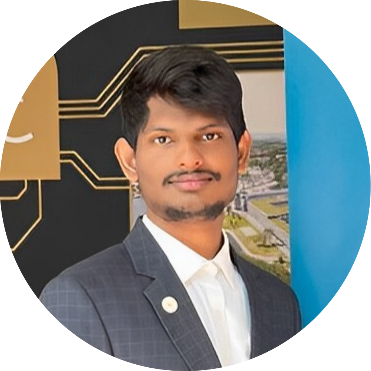
\includegraphics[width=2.7cm,clip]{images/resume_pic_m.png}}
}
\parbox{\dimexpr\linewidth-3.8cm\relax}{
\vspace{-20pt}
\begin{tabularx}{\linewidth}{L r} \\
    {\Huge \scshape  Venkata Sai Yakkshit Reddy Asodi}~\\
    Berlin, Germany. \\ \vspace{1pt}
     \small \raisebox{-0.1\height}\faPhone\ +91 8179936156 ~ \href{mailto:saiyakkshit2001@gmail.com}{\raisebox{-0.2\height}\faEnvelope\  {saiyakkshit2001@gmail.com}} ~ 
    \href{https://linkedin.com/in/yakkshit/}{\raisebox{-0.2\height}\faLinkedin\ {yakkshit}}  ~
    \href{https://yakkshit.com/}{\raisebox{-0.2\height}\faGlobe\ {yakkshit.com}}  ~
    \href{https://github.com/yakkshit}{\raisebox{-0.2\height}\faGithub{ yakkshit}}
    \vspace{-8pt}
\end{tabularx}
}
\end{center}

\vspace{-23pt}
\section{Summary}
Experienced Full Stack Engineer with a passion for Flutter development and soccer. Expertise in building scalable and user-friendly applications with a focus on UI/UX. Skilled in working with international teams and solving real-world challenges for clients in a dynamic, startup environment.

\section{Technical Skills}
\begin{itemize}[leftmargin=0.15in, label={}]
\small{\item{
\textbf{Frameworks - }{Flutter, Riverpod, React, Next.js, Figma.} \\
\textbf{Languages - }{Dart, JavaScript, HTML, CSS, Python.} \\
\textbf{Tools - }{Git, GitHub, Build\_Runner, JSON APIs.} \\
\textbf{Testing - }{Unit, Widget, Integration Tests in Flutter.} \\
\textbf{Deployment - }{App Store, Google Play, Azure, AWS.}
}}
\end{itemize}

\section{Experience}

\resumeSubHeadingListStart

\resumeSubheading
{\large Circleup AG}{Dec 2023 -- July 2024}
  {Lead Full Stack Engineer (Frontend Focus)}{Zurich, Switzerland}\\
\vspace{5pt}
\textbf{Responsibilities:}
\begin{itemize}[leftmargin=0.15in, label={}]
\item Developed interactive, user-friendly mobile apps for soccer team management using Flutter.
\item Managed state with Riverpod and utilized code generation with build\_runner tools.
\item Published fully tested apps to the App Store and Google Play with integration of RESTful JSON APIs.
\item Collaborated with product teams to optimize performance and improve the platform's UI/UX design.
\end{itemize}

\resumeSubheading
{Cedzlabs}{Mar 2023 -- Dec 2023}
{Full Stack Developer}{Remote}\\
\vspace{5pt}
\textbf{Responsibilities:}
\begin{itemize}[leftmargin=0.15in, label={}]
\item Built responsive web applications using React and Flutter with a focus on client requirements.
\item Integrated cloud-based APIs and implemented Agile methodologies to deliver projects on time.
\item Worked on various projects, focusing on accessibility, clean code, and performance.
\end{itemize}

\section{Projects}

\resumeProjectHeading
{\textbf{Coachbetter Soccer App} $|$ \emph{Flutter, Riverpod, Dart, JSON APIs}}{Ongoing}\\
\resumeItemListStart
\vspace{4pt}
\resumeItem
{Developed a 360° soccer training and management app, allowing coaches to plan, organize, and manage teams seamlessly. Integrated real-time data synchronization, team performance analytics, and player statistics tracking.}
\resumeItemListEnd
\vspace{4pt}
\textbf{Tools:}\emph{Flutter, Ios, Android, SQL.}
\vspace{-10pt}

\resumeProjectHeading
{\textbf{AI Resume Generator} $|$ \emph{Next.js, TailwindCSS, LLMs}}{Aug 2023}\\
\resumeItemListStart
\vspace{4pt}
\resumeItem{Created a dynamic AI-powered resume generator that allows users to generate tailored resumes based on inputted details. The tool uses LLMs to fine-tune resume formats for specific job applications.}
\resumeItemListEnd
\vspace{4pt}
\textbf{Tools:}\emph{Nextjs, RAG, React, SQL.}
\vspace{-10pt}

\section{Achievements / Extracurricular / Contributions}
\begin{itemize}[leftmargin=0.15in, label={}]
\item Published apps on both the App Store and Google Play, receiving positive user feedback.
\item Successfully contributed to open-source Flutter projects, enhancing community resources.
\item Participated in tech meetups and workshops focused on Flutter, UI/UX best practices.
\end{itemize}

\end{document}